\documentclass[14pt]{extbook}
\usepackage{multicol, enumerate, enumitem, hyperref, color, soul, setspace, parskip, fancyhdr} %General Packages
\usepackage{amssymb, amsthm, amsmath, bbm, latexsym, units, mathtools} %Math Packages
\everymath{\displaystyle} %All math in Display Style
% Packages with additional options
\usepackage[headsep=0.5cm,headheight=12pt, left=1 in,right= 1 in,top= 1 in,bottom= 1 in]{geometry}
\usepackage[usenames,dvipsnames]{xcolor}
\usepackage{dashrule}  % Package to use the command below to create lines between items
\newcommand{\litem}[1]{\item#1\hspace*{-1cm}\rule{\textwidth}{0.4pt}}
\pagestyle{fancy}
\lhead{Progress Quiz 8}
\chead{}
\rhead{Version A}
\lfoot{4553-3922}
\cfoot{}
\rfoot{Fall 2020}
\begin{document}

\begin{enumerate}
\litem{
Describe the end behavior of the polynomial below.\[ f(x) = 3(x - 5)^{5}(x + 5)^{10}(x + 2)^{2}(x - 2)^{4} \]\begin{enumerate}[label=\Alph*.]
\begin{multicols}{2}\item 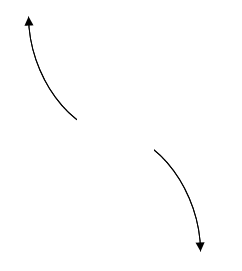
\includegraphics[width = 0.3\textwidth]{../Figures/polyEndBehaviorAA.png}\item 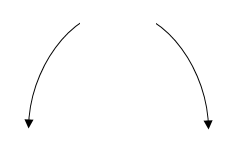
\includegraphics[width = 0.3\textwidth]{../Figures/polyEndBehaviorBA.png}\item 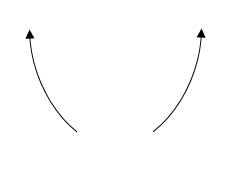
\includegraphics[width = 0.3\textwidth]{../Figures/polyEndBehaviorCA.png}\item 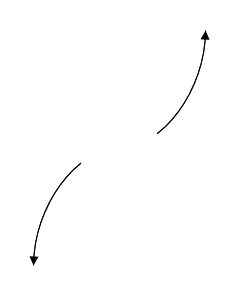
\includegraphics[width = 0.3\textwidth]{../Figures/polyEndBehaviorDA.png}\end{multicols}\item None of the above.
\end{enumerate} }
\litem{
Construct the lowest-degree polynomial given the zeros below. Then, choose the intervals that contain the coefficients of the polynomial in the form $ax^3+bx^2+cx+d$.\[ 2, \frac{7}{5}, \text{ and } \frac{-7}{4} \]\begin{enumerate}[label=\Alph*.]
\item \( a \in [16, 26], b \in [99, 104], c \in [169, 183], \text{ and } d \in [92, 109] \)
\item \( a \in [16, 26], b \in [30, 36], c \in [-66, -61], \text{ and } d \in [-98, -94] \)
\item \( a \in [16, 26], b \in [43, 48], c \in [-40, -34], \text{ and } d \in [-98, -94] \)
\item \( a \in [16, 26], b \in [-44, -31], c \in [-66, -61], \text{ and } d \in [92, 109] \)
\item \( a \in [16, 26], b \in [-44, -31], c \in [-66, -61], \text{ and } d \in [-98, -94] \)

\end{enumerate} }
\litem{
Describe the zero behavior of the zero $x = -2$ of the polynomial below.\[ f(x) = 7(x - 6)^{11}(x + 6)^{8}(x - 2)^{4}(x + 2)^{3} \]\begin{enumerate}[label=\Alph*.]
\begin{multicols}{2}\item 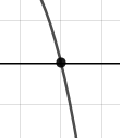
\includegraphics[width = 0.3\textwidth]{../Figures/polyZeroBehaviorCopyAA.png}\item 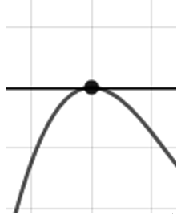
\includegraphics[width = 0.3\textwidth]{../Figures/polyZeroBehaviorCopyBA.png}\item 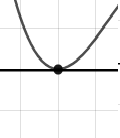
\includegraphics[width = 0.3\textwidth]{../Figures/polyZeroBehaviorCopyCA.png}\item 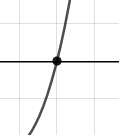
\includegraphics[width = 0.3\textwidth]{../Figures/polyZeroBehaviorCopyDA.png}\end{multicols}\item None of the above.
\end{enumerate} }
\litem{
Construct the lowest-degree polynomial given the zeros below. Then, choose the intervals that contain the coefficients of the polynomial in the form $x^3+bx^2+cx+d$.\[ -3 - 5 i \text{ and } 2 \]\begin{enumerate}[label=\Alph*.]
\item \( b \in [0.5, 3.6], c \in [1.5, 3.3], \text{ and } d \in [-13, -9] \)
\item \( b \in [-4.5, -1.5], c \in [17.2, 24.6], \text{ and } d \in [67, 70] \)
\item \( b \in [0.5, 3.6], c \in [-0.3, 2.4], \text{ and } d \in [-8, 2] \)
\item \( b \in [3.9, 4.8], c \in [17.2, 24.6], \text{ and } d \in [-74, -62] \)
\item \( \text{None of the above.} \)

\end{enumerate} }
\litem{
Which of the following equations \textit{could} be of the graph presented below?
\begin{center}
    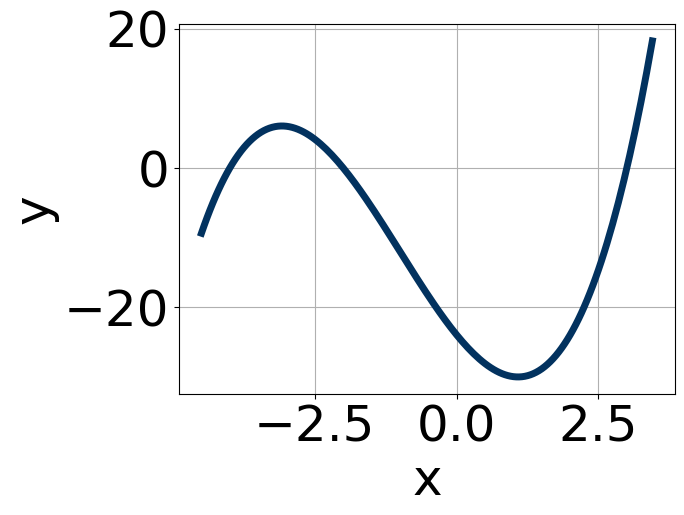
\includegraphics[width=0.5\textwidth]{../Figures/polyGraphToFunctionCopyA.png}
\end{center}
\begin{enumerate}[label=\Alph*.]
\item \( -15x^{8} (x + 2)^{6} (x + 3)^{6} \)
\item \( -16x^{7} (x + 2)^{6} (x + 3)^{10} \)
\item \( 7x^{9} (x + 2)^{10} (x + 3)^{10} \)
\item \( 9x^{8} (x + 2)^{6} (x + 3)^{9} \)
\item \( 15x^{9} (x + 2)^{6} (x + 3)^{5} \)

\end{enumerate} }
\litem{
Describe the zero behavior of the zero $x = 7$ of the polynomial below.\[ f(x) = 2(x - 7)^{9}(x + 7)^{14}(x - 8)^{8}(x + 8)^{11} \]\begin{enumerate}[label=\Alph*.]
\begin{multicols}{2}\item 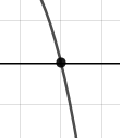
\includegraphics[width = 0.3\textwidth]{../Figures/polyZeroBehaviorAA.png}\item 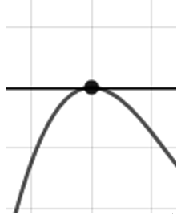
\includegraphics[width = 0.3\textwidth]{../Figures/polyZeroBehaviorBA.png}\item 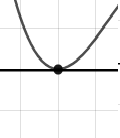
\includegraphics[width = 0.3\textwidth]{../Figures/polyZeroBehaviorCA.png}\item 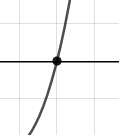
\includegraphics[width = 0.3\textwidth]{../Figures/polyZeroBehaviorDA.png}\end{multicols}\item None of the above.
\end{enumerate} }
\litem{
Describe the end behavior of the polynomial below.\[ f(x) = 8(x - 5)^{3}(x + 5)^{4}(x - 9)^{4}(x + 9)^{4} \]\begin{enumerate}[label=\Alph*.]
\begin{multicols}{2}\item 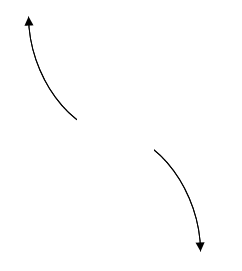
\includegraphics[width = 0.3\textwidth]{../Figures/polyEndBehaviorCopyAA.png}\item 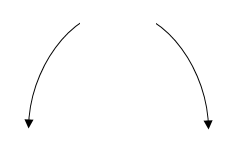
\includegraphics[width = 0.3\textwidth]{../Figures/polyEndBehaviorCopyBA.png}\item 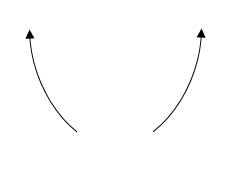
\includegraphics[width = 0.3\textwidth]{../Figures/polyEndBehaviorCopyCA.png}\item 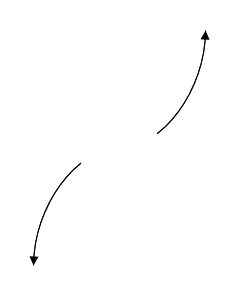
\includegraphics[width = 0.3\textwidth]{../Figures/polyEndBehaviorCopyDA.png}\end{multicols}\item None of the above.
\end{enumerate} }
\litem{
Construct the lowest-degree polynomial given the zeros below. Then, choose the intervals that contain the coefficients of the polynomial in the form $x^3+bx^2+cx+d$.\[ 5 - 2 i \text{ and } 3 \]\begin{enumerate}[label=\Alph*.]
\item \( b \in [-5, 5], c \in [-10, -7], \text{ and } d \in [10, 18] \)
\item \( b \in [-19, -8], c \in [57, 68], \text{ and } d \in [-88, -85] \)
\item \( b \in [-5, 5], c \in [-1, 0], \text{ and } d \in [-14, 2] \)
\item \( b \in [13, 15], c \in [57, 68], \text{ and } d \in [82, 95] \)
\item \( \text{None of the above.} \)

\end{enumerate} }
\litem{
Construct the lowest-degree polynomial given the zeros below. Then, choose the intervals that contain the coefficients of the polynomial in the form $ax^3+bx^2+cx+d$.\[ \frac{-2}{5}, \frac{4}{5}, \text{ and } \frac{-3}{2} \]\begin{enumerate}[label=\Alph*.]
\item \( a \in [48, 53], b \in [51, 63], c \in [-47, -44], \text{ and } d \in [-25, -20] \)
\item \( a \in [48, 53], b \in [15, 17], c \in [-76, -71], \text{ and } d \in [20, 33] \)
\item \( a \in [48, 53], b \in [94, 96], c \in [10, 19], \text{ and } d \in [-25, -20] \)
\item \( a \in [48, 53], b \in [-61, -54], c \in [-47, -44], \text{ and } d \in [20, 33] \)
\item \( a \in [48, 53], b \in [51, 63], c \in [-47, -44], \text{ and } d \in [20, 33] \)

\end{enumerate} }
\litem{
Which of the following equations \textit{could} be of the graph presented below?
\begin{center}
    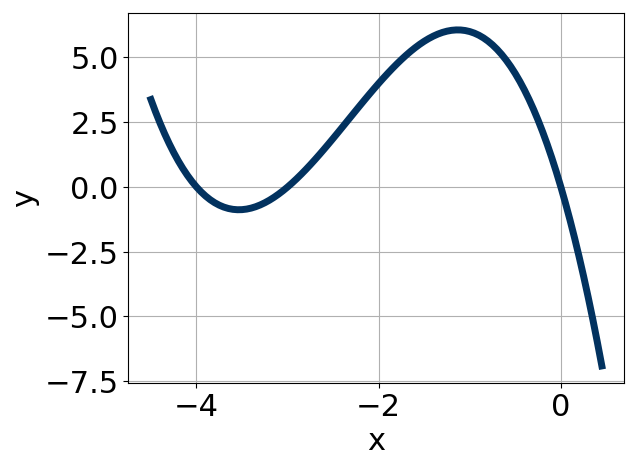
\includegraphics[width=0.5\textwidth]{../Figures/polyGraphToFunctionA.png}
\end{center}
\begin{enumerate}[label=\Alph*.]
\item \( -14(x - 2)^{9} (x + 2)^{7} (x + 1)^{11} \)
\item \( -15(x - 2)^{10} (x + 2)^{8} (x + 1)^{7} \)
\item \( -9(x - 2)^{6} (x + 2)^{7} (x + 1)^{9} \)
\item \( 18(x - 2)^{10} (x + 2)^{9} (x + 1)^{9} \)
\item \( 19(x - 2)^{5} (x + 2)^{5} (x + 1)^{11} \)

\end{enumerate} }
\end{enumerate}

\end{document}